\chapter{Perancangan}
\label{chap:perancangan}

Bab ini membahas perancangan untuk seluruh fitur yang diimplementasi pada  perangkat lunak SharIF Judge.

\section{Tampilan Antarmuka}
\label{sec:4:antarmuka}

\begin{figure}[H]
	\centering  
	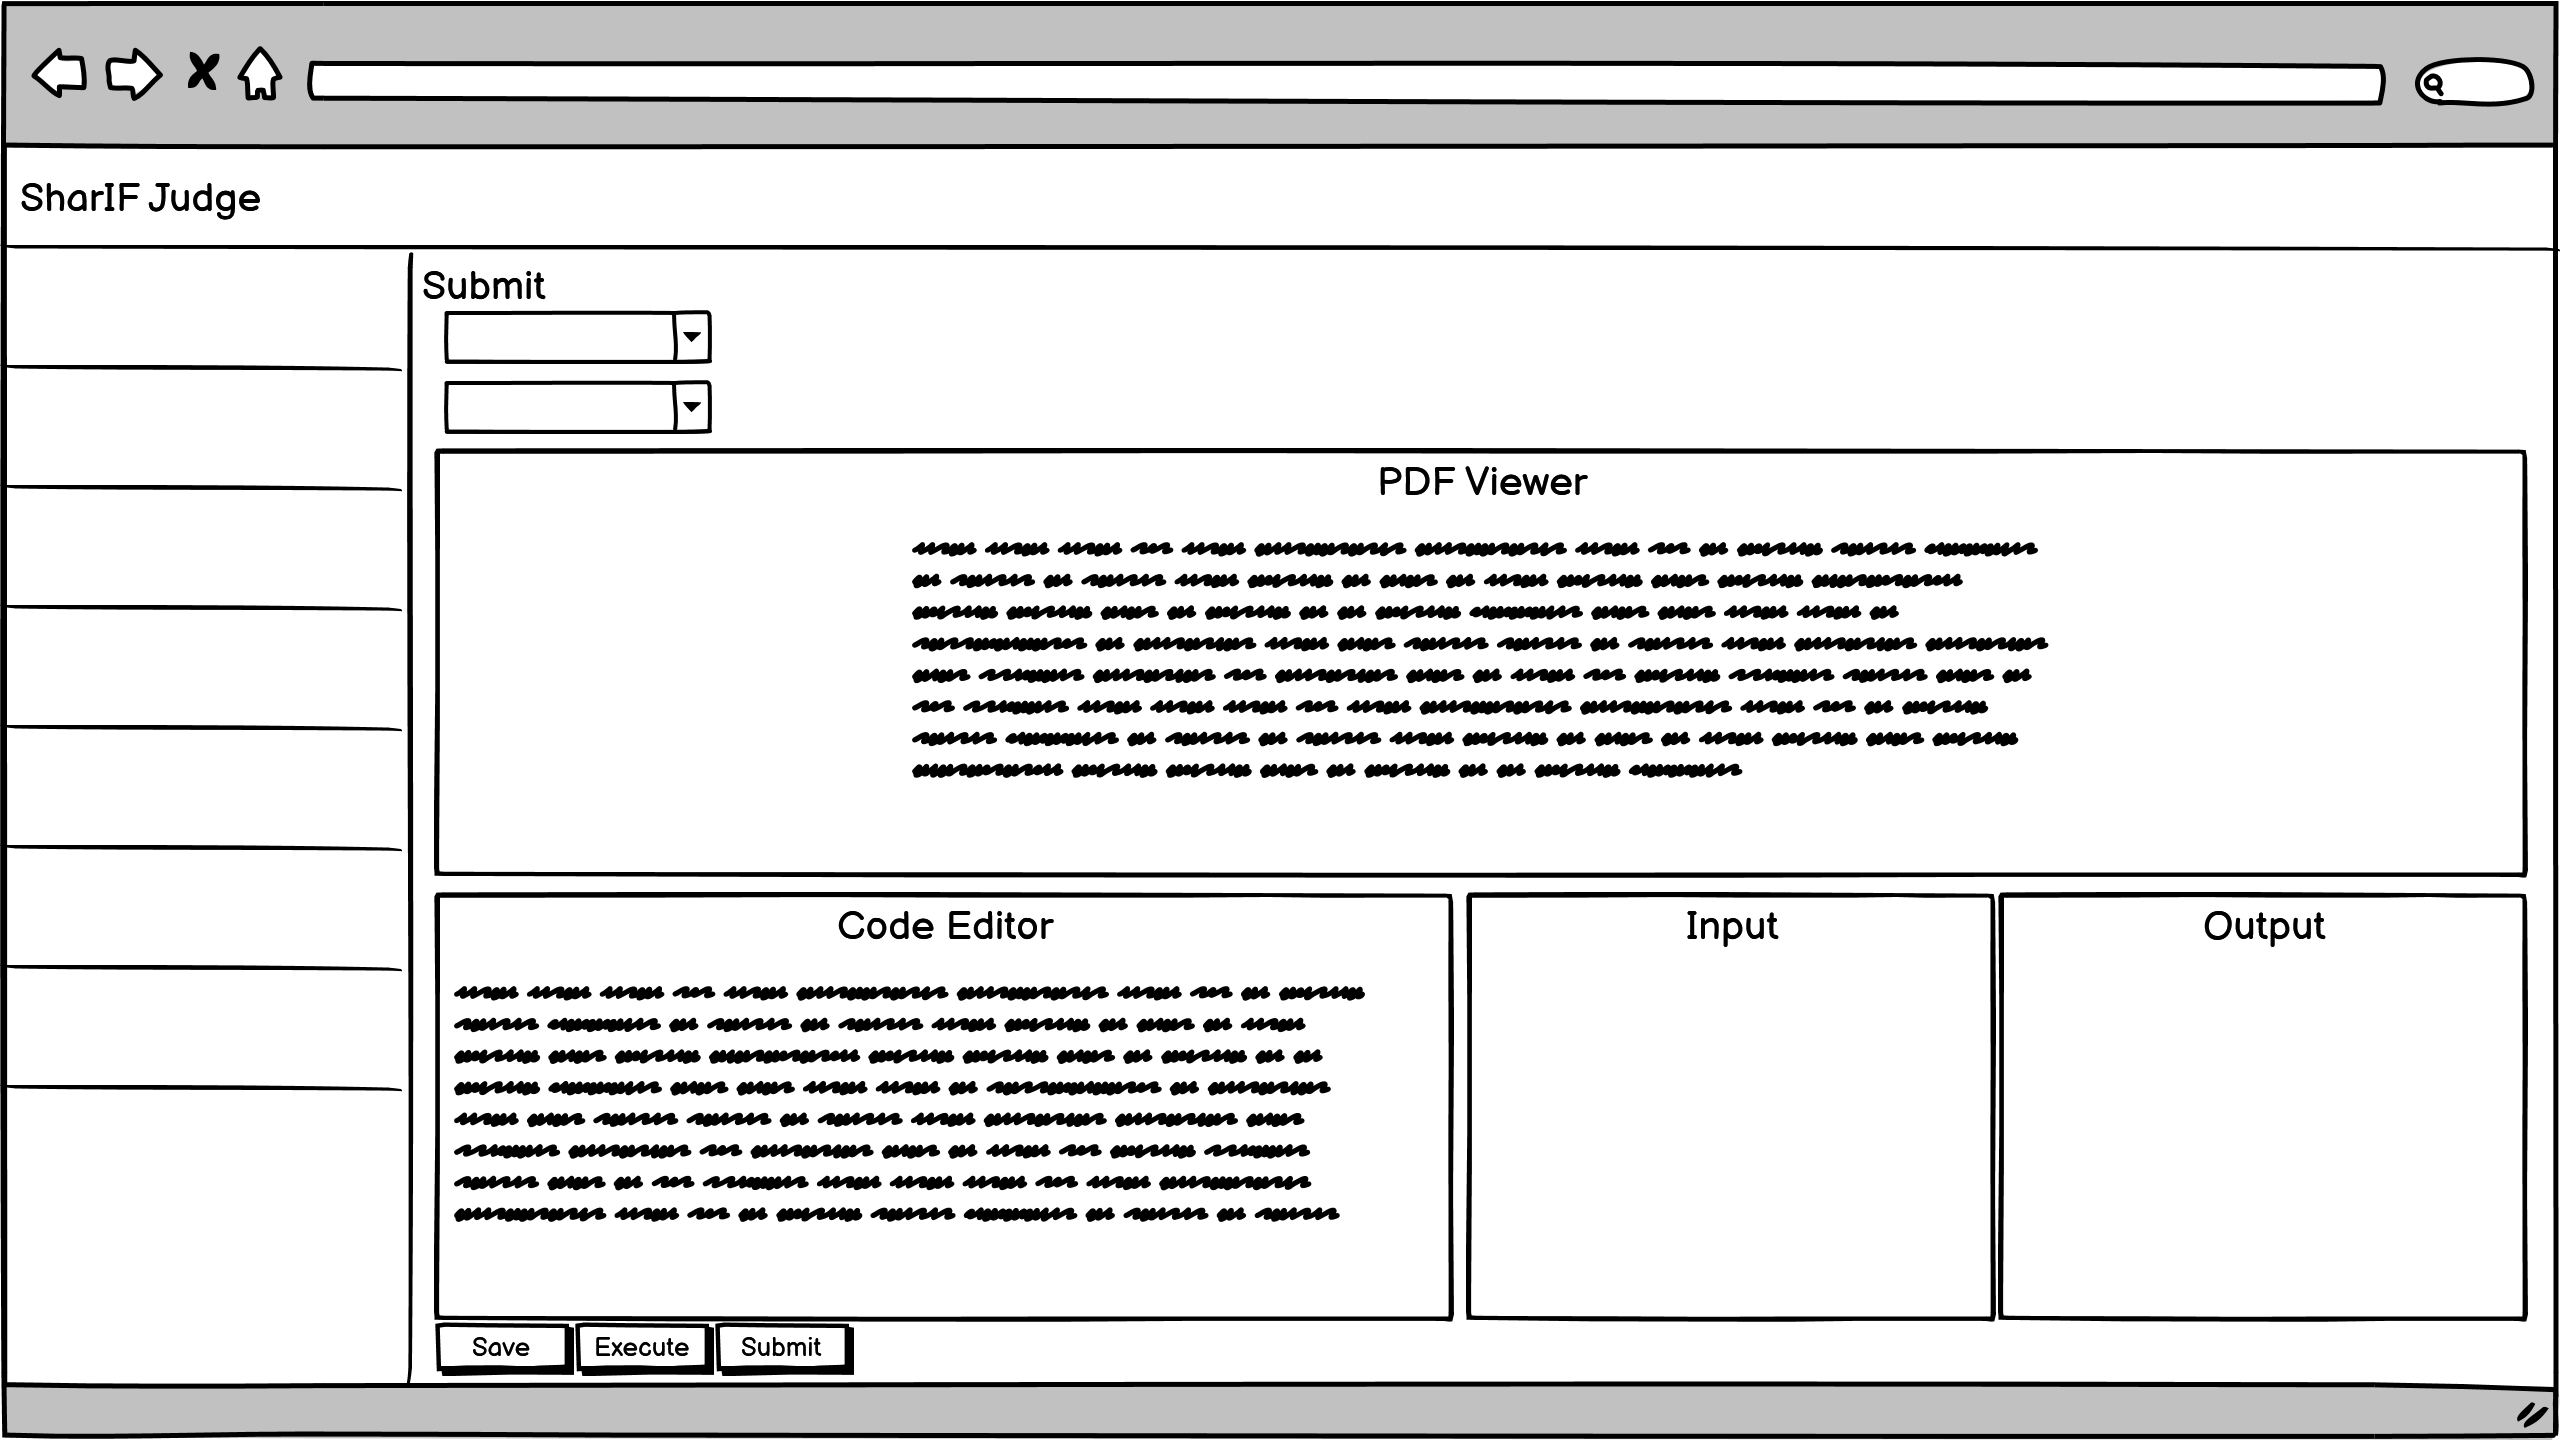
\includegraphics[scale=0.45]{submit mockup}  
	\caption{Rancangan antarmuka halaman Submit} 
	\label{fig:4:antarmuka} 
\end{figure} 

Seluruh fitur akan diimplementasikan pada halaman Submit. Gambar \ref{fig:4:antarmuka} menunjukkan rancangan antarmuka halaman Submit. Pada halaman Submit sudah terdapat \textit{dropdown} untuk memilih \textit{problem} yang akan dikerjakan, dan bahasa pemrograman yang akan digunakan. Kedua \textit{dropdown} tersebut juga akan digunakan pada fitur yang akan diimplementasikan untuk memilih kode \textit{problem} yang akan disimpan dan dimuat, serta memilih mode \textit{syntax highlighting} pada editor kode.

\section{Menampilkan soal}
\label{sec:4:soal}

SharIF Judge sudah memiliki kemampuan untuk menyimpan soal dalam bentuk PDF, namun untuk melihat soal tersebut, soal harus diunduh terlebih dahulu. Agar pengguna dapat melihat soal secara langsung di halaman \textit{web}, digunakan \textit{library} PDF.js untuk menampilkan \textit{file} PDF soal di halaman Submit. Fungsi \verb|pdf| pada \textit{controller} \verb|Assignments| berfungsi untuk mengembalikan \textit{file} PDF soal untuk \textit{assignment} tertentu. 

Untuk menampilkan soal PDF pada halaman Submit, perlu dilakukan perubahan sebagai berikut:
\begin{itemize}
    \item Penambahan \verb|iframe| pada \textit{view} Submit untuk menampilkan PDF.js.
    \item Perubahan pada fungsi \verb|pdf| agar \textit{file} PDF dapat dibaca dan ditampilkan oleh PDF.js, dan tidak menampilkan dialog unduh \textit{file}.
\end{itemize}

\section{Editor Kode}
\label{sec:4:editor}

Untuk menambahkan editor kode pada halaman Submit, digunakan \textit{library} Ace. Seluruh konfigurasi untuk menampilkan editor Ace dilakukan pada JavaScript.

Untuk menambahkan editor kode pada halaman Submit, perlu dilakukan perubahan sebagai berikut:
\begin{itemize}
    \item Penambahan \verb|div| pada \textit{view} Submit untuk menampilkan editor Ace.
    \item Penambahan fungsi JavaScript pada \textit{view} Submit untuk menampilkan editor Ace dan menyesuaikan mode \textit{syntax highlighting} pada editor kode dengan pilihan bahasa pemrograman pada \textit{dropdown}.
\end{itemize}

\section{Menyimpan Kode}
\label{sec:4:simpan}

Seluruh \textit{submission} yang diunggah oleh pengguna  pada SharIF Judge akan disimpan pada folder \verb|Assignments| sesuai dengan \textit{assignment} dan \textit{problem} yang dipilih. Kode pada editor kode juga akan disimpan pada folder yang sama sebagai sebuah \textit{file} txt. 

Untuk menyimpan dan mengambil kode pada editor kode, perlu dilakukan perubahan sebagai berikut:
\begin{itemize}
    \item Penambahan fungsi pada \textit{controller} \verb|Submit| untuk menyimpan kode sebagai \textit{file} txt.
    \item Penambahan fungsi JavaScript pada \textit{view} Submit untuk mengambil kode yang sudah tersimpan saat memilih \textit{problem} pada \textit{dropdown}, dan menyimpan kode yang tedapat di editor kode ketika tombol Save ditekan.
\end{itemize}

\section{Menjalankan Kode dengan Tes Kasus}
\label{sec:4:jalan}

Pada SharIF Judge, seluruh kode yang di\textit{submit} pengguna akan dijalankan satu per satu dalam antrian untuk dinilai. Tahap-tahap yang dilalui sebuah kode hingga penilaian selesai adalah sebagai berikut:
\begin{itemize}
    \item \textit{File} kode disimpan pada folder sesuai dengan \textit{assignment} dan \textit{problem} yang dipilih.
    \item Kode dimasukkan dalam antrian sebagai sebuah \textit{entry} di \textit{database} \verb|queue|.
    \item Kode dijalankan pada \verb|tester.sh| sesuai antrian untuk dikompilasi satu per satu lalu dijalankan dengan tes kasus yang disediakan untuk menghasilkan nilai.
    \item Nilai disimpan pada database \verb|submissions| dan dihapus dari antrian.
\end{itemize}

Untuk menjalankan kode dari editor kode, akan dimanfaatkan sistem antrian yang sudah tersedia. Untuk memasukkan kode dari editor kode ke antrian, diperlukan perubahan sebagai berikut:
\begin{itemize}
    \item Penambahan \verb|textarea| pada \textit{view} Submit untuk \textit{input} dan \textit{output}.
    \item Penambahan fungsi pada \textit{controller} \verb|Submit| untuk menyimpan kode dari editor dan mengambil hasil dari eksekusi kode.
    \item Penambahan fungsi pada \textit{controller} \verb|Queue| untuk memasukkan kode dari editor ke antrian.
    \item Penambahan fungsi pada \textit{controller} \verb|Queueprocess| untuk menangani eksekusi kode tanpa penilaian.
    \item Perubahan pada \verb|tester.sh| untuk mengembalikan \textit{output} dari kode tanpa perlu melakukan penilaian.
\end{itemize}